\documentclass[conference]{IEEEtran}
\IEEEoverridecommandlockouts

\usepackage{amsmath,amsfonts,amssymb,bm}
\usepackage{algorithmic}
\usepackage{algorithm}
\usepackage{array}
\usepackage{booktabs}
\usepackage{multirow}
\usepackage{textcomp}
\usepackage{url}
\usepackage{graphicx}
\usepackage{cite}
\usepackage{xcolor}

\hyphenation{op-tical net-works semi-conduc-tor IEEE-Xplore}

% -----------------------------------------------------------------------------
% Draft controls. Set \draftnotesfalse before submission and resolve every note.
% Numbers come from the frozen runs listed in docs/copl/claude_notes/04 (Sec. 8) and
% must not be edited by hand; regenerate the tables from the run artifacts instead.
% -----------------------------------------------------------------------------
\newif\ifdraftnotes
\draftnotestrue
\newcommand{\draftnote}[1]{\ifdraftnotes\textcolor{red}{\textbf{[TODO: #1]}}\fi}

\newcommand{\R}{\mathbb{R}}
\newcommand{\E}{\mathbb{E}}
\newcommand{\Var}{\operatorname{Var}}
\newcommand{\sigmoid}{\sigma}
\newcommand{\D}{\mathcal{D}}
\newcommand{\newuser}{\star}
\newcommand{\method}{CoPL-LP}
\newcommand{\T}{\mathsf{T}}

\begin{document}

\title{Who Is This Occupant? Likelihood-Based User Posteriors for Few-Label Personalization of Ride-Comfort Judgments\\
\draftnote{Alternative titles in claude\_notes/04, Sec.~1; choose one.}}

\author{\IEEEauthorblockN{Jaewoong Han, Sheengil Kang, and Jongeun Choi}
\IEEEauthorblockA{\draftnote{Affiliations, e-mail addresses, corresponding author, funding.}}}

\maketitle

\begin{abstract}
Whether a vehicle's response to a road bump feels good or bad differs between occupants, and a new occupant supplies only a few binary labels. Collaborative preference learning (CoPL) addresses this cold start by embedding users and labeled items in a shared graph, training a reward model conditioned on the user embedding, and adapting to a new user at test time by voting the user's labels over the graph and mixing the embeddings of the population users. We transfer this recipe to in-vehicle ride feedback and find that the test-time vote fails there: because every episode belongs to one occupant, the user--item graph is a union of stars, the vote score of a population user grows with the number of that user's labels, and the adaptation weights drift to the most-labeled occupant regardless of agreement. Normalizing or shrinking the vote only moves the bias to the least-labeled occupants. We replace the vote by a tempered posterior over population users computed from the reward model's own likelihood of the new occupant's labels. The rule needs no item graph, has no degree bias, accumulates evidence with the number of labels, and costs one forward pass per population user and label. In a leave-one-occupant-out evaluation on 2682 real-vehicle bump episodes from 18 occupants, the likelihood posterior improves the held-out log predictive density after 20 labels by 0.08 nat per episode over a calibrated pooled classifier fine-tuned on the same labels (two occupant-level standard errors) and by 0.09 nat over the graph vote, while matching the pooled classifier at the cold start. Item--item propagation in the graph and the sparsification of the item graph have no measurable effect, and a fixed Gabor-scattering encoder outperforms learned autoencoders as the item representation.
\end{abstract}

\begin{IEEEkeywords}
collaborative filtering, few-shot personalization, human feedback, intelligent vehicles, preference learning, ride comfort.
\end{IEEEkeywords}

\section{Introduction}
\label{sec:intro}

Ride comfort is judged by the occupant, and occupants disagree. Objective ride metrics summarize the vehicle response to a road input~\cite{guastadisegni2024ride,iso2631}, and data-driven evaluators map such responses to a population-level comfort score~\cite{cieslak2020ride,kim2019evaluator}, but an adaptive chassis that wants to please the person in the seat needs that person's judgment, and the person will not label hundreds of bumps before the system adapts. The practical setting is therefore few-label personalization: predict whether a particular occupant will judge the next bump response as good or bad, given a population of previous occupants' good/bad feedback and a handful of labels from the new occupant.

Collaborative filtering is the natural framework for borrowing other users' labels, and collaborative preference learning (CoPL)~\cite{choi2025copl} packages it for preference data: users and labeled items form a bipartite graph with good and bad edges, a graph convolution~\cite{he2020lightgcn} produces user and item embeddings, a reward model conditioned on the user embedding predicts the label of any item, and a new user is adapted at test time by attaching the user's labeled items to their nearest neighbors in the graph, voting over the population users, and mixing the population embeddings with the softmax of the votes. The user embedding plays the role that occupant-specific parameters would play in a parametric model, and the mixture is the cold-start mechanism.

Transferring this recipe to ride feedback exposes a structural difference from recommendation data. Each bump episode is experienced and labeled by exactly one occupant, so the user--item graph is a disjoint union of stars and carries no path between users; the only cross-user edges are those of an item--item similarity graph computed from the episode waveforms. The vote that adapts a new user is a sum over the items of each population user of the votes that reached them, and it therefore scales with how many items the user has. In our data this is not a second-order effect: for every one of ten held-out occupants the adaptation weight concentrated on the population occupant with the most labels, and the occupant with the longest stream was adapted to a population occupant whose base rate of good judgments differs from hers by 35 percentage points, which made the personalized prediction worse than no personalization at all. Normalizing the vote by the number of items, or shrinking it with a pseudo-count, moves the bias from the largest to the smallest occupants without removing it.

This paper makes three contributions.
\begin{enumerate}
  \item We analyze why the CoPL test-time vote fails on star-structured feedback data: the user score has a degree bias, and the family of normalized and shrunken votes contains no member that works across occupants, because the vote measures label agreement only through a nearest-neighbor proxy (Section~\ref{sec:vote}).
  \item We replace the vote by a likelihood-based user posterior: the reward model itself scores how probable the new occupant's labels are under each population user's embedding, and a tempered softmax of these log-likelihoods mixes the embeddings (Section~\ref{sec:posterior}). The rule uses no graph, has no degree bias, sharpens with the number of labels, and is exact Bayesian model averaging over population users at unit temperature.
  \item We evaluate both rules and three baselines under a leave-one-occupant-out protocol on 2682 real-vehicle bump episodes from 18 occupants, with context budgets of 0 to 20 labels and occupant-level standard errors (Section~\ref{sec:experiments}). The likelihood posterior improves the held-out log predictive density after 20 labels by $0.08$ nat over a calibrated pooled classifier fine-tuned on the same labels and by $0.09$ nat over the vote; ablations show that item--item propagation in the graph contributes nothing, that training the reward model on mixed embeddings and calibrating it are necessary, and that a fixed scattering encoder is a better item representation than learned autoencoders.
\end{enumerate}

\section{Related Work}
\label{sec:related}

\textbf{Ride comfort and its personalization.} Objective ride evaluation relates body-motion statistics and frequency-weighted exposure~\cite{iso2631} to subjective ratings~\cite{guastadisegni2024ride,elbanhawi2015passenger}; learned evaluators regress ratings or classify bump responses from accelerometer signals~\cite{cieslak2020ride,kim2019evaluator}. Personalization has been approached by sensory profiling of individuals~\cite{kikuchi2025personalizing} and by online preference learning for driving style~\cite{ran2023online,bae2020robocar}. These works either fit one model per person from that person's data or tune a population model; none transfers the labels of previous occupants to a new one with a handful of labels.

\textbf{Preference learning from human feedback.} Reward models trained from human comparisons~\cite{christiano2017deep} and active elicitation of preferences~\cite{sadigh2017active} assume a single reward function. Multi-user extensions learn a latent user variable: hierarchical Gaussian-process preference learning~\cite{birlutiu2013efficiently} and variational preference learning~\cite{poddar2024vpl} infer a user context from the user's own labels. CoPL~\cite{choi2025copl} instead obtains user representations from a user--item graph by collaborative filtering and adapts a new user by a graph vote; we keep its training pipeline and replace the adaptation.

\textbf{Cold start and model averaging.} The cold-start problem of collaborative filtering is classical~\cite{schein2002coldstart,koren2009matrix}. Our adaptation treats the identity of the new occupant among the population occupants as a discrete latent variable and averages the reward model over its posterior, which is Bayesian model averaging~\cite{hoeting1999bma}. Because the population users are not the new user, the posterior is misspecified, and we temper it; the generalized posterior framework~\cite{bissiri2016general} and the safe-Bayes analysis of misspecified models~\cite{grunwald2017inconsistency} give the rationale for a learning rate below one. The likelihood scores are meaningful only if the reward model's probabilities are calibrated~\cite{guo2017calibration,vancalster2019calibration}, which is why calibration appears in the ablation.

\section{Problem Setting and the Collaborative Pipeline}
\label{sec:pipeline}

\subsection{Binary Ride Feedback and the Prediction Task}
\label{sec:setting}

A bump episode is a window of vehicle motion signals $x\in\R^{C\times T}$ ($C$ channels, $T$ samples) around a detected road input, and its label $y\in\{0,1\}$ records whether the occupant judged the response good ($y=1$) or bad ($y=0$). A population of $U$ occupants has labeled $\D_{1:U}=\{(x_{ui},y_{ui})\}$, where occupant $u$ labeled items $I_u$ with $n_u=|I_u|$. A new occupant $\newuser$ has labeled a context $\D_{\newuser,t}=\{(x_{\newuser i},y_{\newuser i})\}_{i\le t}$ of $t$ episodes in the order in which they occurred. The task is to predict, for a pending episode $j$,
\begin{equation}
 p(y_{\newuser j}=1\mid x_{\newuser j},\D_{\newuser,t},\D_{1:U}),
 \label{eq:target}
\end{equation}
at every context size $t$ from the cold start $t=0$ upward. The prediction is scored by the log predictive density on episodes the occupant has not yet labeled, so a model is rewarded for calibrated probabilities, not only for ranking.

The structural property that drives this paper follows from the data collection: an episode is experienced by one occupant and labeled by that occupant only. The user--item relation is therefore a function from items to users, the bipartite graph of users and items is a disjoint union of stars (Fig.~\ref{fig:overview}A), and no two users share an item. Any transfer of labels between users must pass through a similarity between items.

\begin{figure*}[t]
\centering
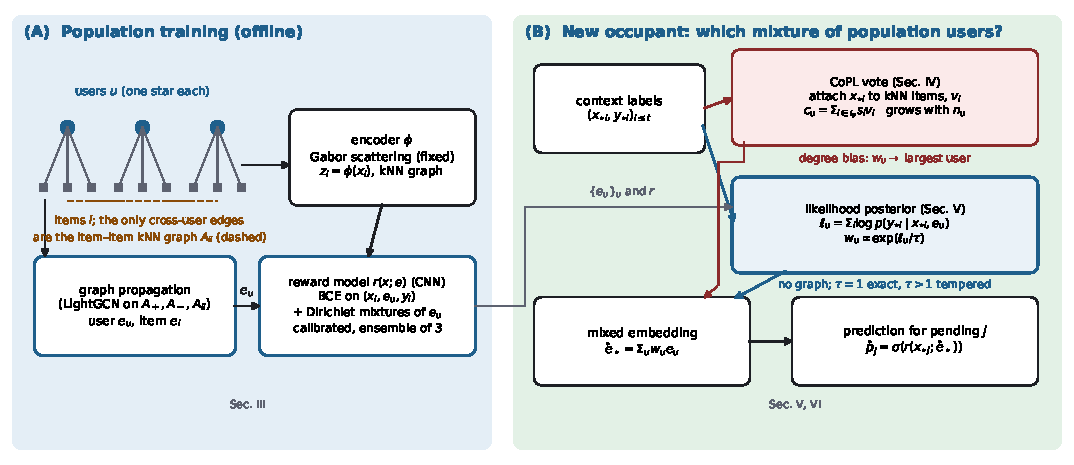
\includegraphics[width=\textwidth]{figures/fig_overview.pdf}
\caption{Overview. (A) Offline, a fixed scattering encoder turns episodes into vectors and a kNN graph; graph propagation over the user--item stars and the item--item graph yields user embeddings $e_u$ and item embeddings; a reward model $r(x;e)$ is trained on the population labels, on Dirichlet mixtures of user embeddings, and is calibrated. (B) Online, a new occupant's context labels are turned into weights $w_u$ over the population users and the mixed embedding $\hat e_\newuser$ conditions the reward model. CoPL's vote (top) scores users by a nearest-neighbor vote that grows with the user's number of items; the proposed rule (bottom) scores users by the reward model's log-likelihood of the context labels.}
\label{fig:overview}
\end{figure*}

\subsection{Item Representation and Item--Item Graph}
\label{sec:encoder}

Each episode is encoded by a fixed map $z=\phi(x)\in\R^{d}$ and connected to its $k$ nearest population episodes in Euclidean distance with Gaussian affinities. We use a Gabor scattering transform~\cite{mallat2012scattering,anden2014deep} per channel: first-order coefficients are the time averages of $|x*\psi_\lambda|$ over a bank of $8$ Gabor filters, second-order coefficients iterate the modulus with a lower-frequency filter, and the coefficients of the $C=5$ channels are concatenated ($d=185$). The transform is translation-invariant over the window, stable to small time warps, and has no trainable parameters, so it is identical for every fold and seed. We chose it from six candidates (principal components, an autoencoder, a variational autoencoder, a bank of ISO-inspired transient statistics, a Gaussian kernel on the raw waveform, and scattering) by a population-only criterion that needs no reward model: the AUROC of a $k$-nearest-neighbor label vote for held-out occupants. Scattering scored $0.72$, the ISO bank $0.61$, the raw kernel $0.59$, and the two learned encoders $0.55$ and $0.54$; reconstruction objectives preserve amplitude and phase variation that the labels do not depend on. The population-only criterion correlates with the final held-out quality across $72$ encoder and channel-subset combinations (Spearman $0.78$), so it is a usable selection rule.

\subsection{Graph Propagation}
\label{sec:gcf}

Let $A_+$ and $A_-$ be the user--item incidence matrices of good and bad labels and $A_{ii}$ the symmetric item--item kNN graph. Following CoPL, user and item embeddings are initialized freely and propagated for two LightGCN-style layers~\cite{he2020lightgcn} over the normalized $A_+$, $A_-$ (with a sign for bad edges), and $A_{ii}$ with weight $\lambda_{ii}$, and trained with a binary cross-entropy on the user--item edges plus a diversity penalty on the cosine similarities between user embeddings. The output is a user embedding $e_u\in\R^{m}$ for every population user and an item embedding $e_i$ for every population item. We will show in Section~\ref{sec:results} that the item--item term contributes nothing on this data; the embeddings $e_u$ are what matters downstream.

\subsection{Reward Model}
\label{sec:rm}

The reward model $r(x;e)$ is a one-dimensional convolutional network: the channels at each time step are projected to a hidden width, the user embedding is projected to the same width and added to every time step, two convolutional layers with kernel size $3$ follow, and a max-pool over time feeds a two-layer head that outputs a logit. It is trained with binary cross-entropy on $(x_{ui},e_u,y_{ui})$ over the population. Three details of the training matter for what follows, and each is ablated in Section~\ref{sec:results}.

\emph{Mixture-consistent training.} At test time the model is queried with convex mixtures of population embeddings (the mean at the cold start, a softmax mixture after adaptation), which are off the training distribution of one-hot users. We therefore replace the embedding of a random half of the training rows by $(1-\lambda)\,e_u+\lambda\sum_{u'}\pi_{u'}e_{u'}$ with $\pi\sim\mathrm{Dirichlet}(\bm 1)$ and $\lambda\sim\mathrm{Uniform}(0,1)$, keeping the label; this is mixup~\cite{zhang2018mixup} in the embedding argument only.

\emph{Calibration.} Model selection uses the validation cross-entropy on a $10\%$ per-user split rather than the validation AUROC, and a temperature is fitted on the same split~\cite{guo2017calibration}. The likelihood-based rule of Section~\ref{sec:posterior} reads the model's probabilities as evidence, so their scale must be right.

\emph{Ensemble.} Three models with different seeds are averaged in probability~\cite{lakshminarayanan2017ensembles}; the ensemble also stabilizes the likelihood scores.

\subsection{Test-Time Adaptation in CoPL}
\label{sec:copl-adapt}

A new occupant is represented by a mixture $\hat e_\newuser=\sum_u w_ue_u$ of the population embeddings, and the prediction is $\hat p_{\newuser j}=\sigmoid(r(x_{\newuser j};\hat e_\newuser))$. At the cold start the weights are uniform. With a context, CoPL computes the weights by a vote. Each context episode is attached to its $k$ nearest population items with affinities $a_{i'i}$, and every attached item accumulates a signed vote,
\begin{equation}
 v_i=\sum_{i'\le t}a_{i'i}\,s_{\newuser i'},\qquad s_{\newuser i'}=\begin{cases}+1 & y_{\newuser i'}=1\\ -\beta & y_{\newuser i'}=0,\end{cases}
 \label{eq:vote-items}
\end{equation}
where $\beta$ weights the bad labels. The score of population user $u$ sums the votes on $u$'s items, signed by $u$'s own labels $s_i\in\{+1,-1\}$, and the weights are a softmax with temperature $\tau$:
\begin{equation}
 c_u=\sum_{i\in I_u}s_i\,v_i,\qquad w_u=\frac{\exp(c_u/\tau)}{\sum_{u'}\exp(c_{u'}/\tau)}.
 \label{eq:vote-users}
\end{equation}
The score rewards users whose labels agree with the new occupant's labels on similar items, which is the intended collaborative signal.

\section{Why the Vote Fails: Degree Bias}
\label{sec:vote}

Write the vote score as a sum over the items of user $u$ and take its expectation over the context,
\begin{equation}
 \E[c_u]=\sum_{i\in I_u}s_i\,\E[v_i]\approx n_u\cdot\overline{(s\,v)}_u,
 \label{eq:degree}
\end{equation}
where $\overline{(s\,v)}_u$ is the mean signed vote per item of user $u$, the quantity that measures agreement. Two users with the same mean agreement receive scores in the ratio of their item counts $n_u$. On recommendation data the item counts of active users are comparable and the bias is mild; on star-structured feedback data where one occupant labeled $1056$ episodes and another $10$, it dominates. Furthermore $c_u$ grows linearly with the context size $t$, so for a long context the softmax is one-hot at any fixed $\tau$, and the one-hot falls on the user with the largest $n_u\,\overline{(sv)}_u$, which for a positive mean agreement is the largest user.

The effect is visible in every fold of our experiment (Fig.~\ref{fig:wu}, left). For all ten held-out occupants the weight at the full context concentrates on the population occupant with the most labels. The longest stream, occupant E1 (41\% good judgments), is adapted entirely to occupant E2 (76\% good) and her held-out log predictive density falls from $-0.72$ at the cold start to $-1.09$ at the full context, far below the pooled classifier ($-0.62$). The reward model is not at fault: conditioning it on E1's own population embedding (an oracle available only in evaluation) gives $-0.55$. The adaptation simply selects the wrong occupant.

\textbf{Normalization and shrinkage do not repair it.} The obvious remedy divides the score by the user's size, $\tilde c_u=c_u\,(\bar n/n_u)^{\alpha}$, with $\alpha=1$ turning the sum into a per-item mean agreement rescaled by the mean size $\bar n$. With $\alpha=1$ occupant E1 is adapted to a small population occupant and reaches $-0.56$, the oracle level, but the per-item mean of an occupant with ten items is noise: occupant E5 is now adapted to the smallest population occupant and falls from $-0.55$ to $-0.72$. The bias has changed sign, not disappeared. A pseudo-count $\kappa$ that shrinks small users toward neutrality, $\tilde c_u=c_u\,(\bar d+\kappa)/(d_u+\kappa)$ with $d_u$ the item count or the vote mass that reached $u$, interpolates between the two regimes, and every value of $\kappa$ we tried ($0.3$ to $3$ times $\bar d$) returned E1 to a large occupant and to $-0.92$ or worse. Over a grid of $36$ settings of $(\alpha,\kappa,d_u,\tau)$ evaluated on all ten folds, no setting kept every fold within $0.02$ nat of the better of the pooled classifier and no adaptation; the best covered eight folds. The requirements of E1 (trust a small occupant) and E5 (do not trust a small occupant) conflict for any statistic that measures agreement through nearest-neighbor attachment, because attachment is a proxy for label agreement, not a measurement of it.

\section{Likelihood-Based User Posterior}
\label{sec:posterior}

The pipeline already contains a direct measurement of agreement: the reward model conditioned on $e_u$ is a probabilistic classifier of what user $u$ would say about any episode. We score each population user by the log-likelihood of the new occupant's context under that user's embedding,
\begin{equation}
 \ell_u(t)=\sum_{i\le t}\Big[y_{\newuser i}\log\sigmoid\big(r(x_{\newuser i};e_u)\big)+(1-y_{\newuser i})\log\big(1-\sigmoid(r(x_{\newuser i};e_u))\big)\Big],
 \label{eq:loglik}
\end{equation}
and set
\begin{equation}
 w_u=\frac{\exp\big(\ell_u(t)/\tau\big)}{\sum_{u'}\exp\big(\ell_{u'}(t)/\tau\big)},\qquad
 \hat e_\newuser=\sum_u w_u\,e_u.
 \label{eq:posterior}
\end{equation}
At $\tau=1$, $w_u$ is the posterior probability that the new occupant is population user $u$ under a uniform prior and the reward model's likelihood, and $\hat e_\newuser$ is the posterior-mean embedding; the prediction $\sigmoid(r(x;\hat e_\newuser))$ is a mixture-in-embedding approximation of Bayesian model averaging over users~\cite{hoeting1999bma}. The approximation is what the mixture-consistent training of Section~\ref{sec:rm} makes legitimate: the model has been trained on exactly such mixtures.

The rule has the properties the vote lacks. It needs no item graph and no nearest-neighbor attachment, so the graph serves only to produce $e_u$. Every user is scored on the same $t$ episodes, so there is no degree bias: a user with ten items and a user with a thousand are compared by how well their embeddings explain the new occupant's labels. The score accumulates with $t$ in units of nats, so the weights sharpen as evidence arrives, as the original vote's scale did, and the sharpening is governed by the model's calibrated probabilities rather than by affinity sums. Its cost is $U\times t$ forward passes of the reward model, which is negligible next to training.

\textbf{Tempering.} The population users are not the new occupant, so the posterior is misspecified and $\tau=1$ can be overconfident on short contexts whose few labels happen to match one user. We treat $\tau$ as a learning rate in the sense of generalized posteriors~\cite{bissiri2016general,grunwald2017inconsistency} and select it, together with whether $\ell_u$ is standardized across users before the softmax, by an inner leave-one-occupant-out search inside each population set (Section~\ref{sec:protocol}). At the cold start $t=0$ the weights are uniform and the rule coincides with CoPL.

\section{Experiments}
\label{sec:experiments}

\subsection{Data}
\label{sec:data}

Episodes were collected in a [vehicle model] driven over speed bumps and similar discrete road inputs on [road description]. \draftnote{Vehicle, road, sensor models, sampling, mounting, recruitment, consent and ethics statement; same items as the companion data description.} Five motion channels enter the model: longitudinal, lateral, and vertical acceleration from the production inertial measurement unit, and bounce (heave) rate and pitch rate from a six-degree-of-freedom body-motion sensor. Each episode is a window from $2$~s before to $2$~s after the detected bump, low-pass filtered at $10$~Hz and downsampled to $50$~Hz ($T=200$), and standardized per channel on the population set of each fold. Immediately after each bump the occupant stated whether the response was good or bad.

Eighteen occupants labeled $2682$ episodes. Ten of them labeled at least $10$ episodes with at least $3$ of each class and take the held-out role in turn; Table~\ref{tab:data} lists them with protocol-local identifiers E1--E10 in order of stream length. The remaining eight occupants labeled $55$ episodes in total and enter every population graph but are never held out. The ten streams are very unequal: five occupants labeled between $205$ and $1056$ episodes, five between $10$ and $35$, which is the regime in which few-label personalization is actually tested.

\begin{table}[t]
\caption{Held-Out Occupants and Episode Counts}
\label{tab:data}
\centering
\setlength{\tabcolsep}{5pt}
\begin{tabular}{lrrrrr}
\toprule
Occupant & Episodes & Good & Bad & $n_{\mathrm{ctx}}$ & $n_{\mathrm{hold}}$ \\
\midrule
E1  & 1056 & 436 & 620 & 528 & 528 \\
E2  &  591 & 452 & 139 & 295 & 296 \\
E3  &  369 & 280 &  89 & 184 & 185 \\
E4  &  279 &  66 & 213 & 139 & 140 \\
E5  &  205 & 128 &  77 & 102 & 103 \\
E6  &   35 &  18 &  17 &  17 &  18 \\
E7  &   34 &  16 &  18 &  17 &  17 \\
E8  &   30 &  14 &  16 &  15 &  15 \\
E9  &   18 &  15 &   3 &   9 &   9 \\
E10 &   10 &   6 &   4 &   5 &   5 \\
\midrule
Total & 2627 & 1431 & 1196 & 1311 & 1316 \\
\bottomrule
\end{tabular}
\\[2pt]
{\footnotesize Eight further occupants with $55$ episodes in total are in the population set only.}
\end{table}

\subsection{Protocol}
\label{sec:protocol}

The protocol is leave-one-occupant-out. For each held-out occupant the other seventeen form the population: the encoder statistics, the item graph, the graph propagation, the reward model, its calibration, and every baseline are fitted on the population only. The held-out stream is split in recorded order into a context half of $n_{\mathrm{ctx}}=\lfloor N/2\rfloor$ episodes, revealed sequentially, and a holdout half on which all metrics are computed. Context budgets follow $t\in\{0,5,10,20,n_{\mathrm{ctx}}\}$, truncated to the stream; each $t<n_{\mathrm{ctx}}$ is evaluated for three starting offsets of the context window, spaced over the context half, and averaged. Macro averages at budget $t$ are over the occupants whose context half has at least $t$ episodes: ten at $t\le5$, eight at $t=10$, five (E1--E5) at $t=20$. Every fold is repeated with three seeds of the graph propagation, the reward models, and the baselines; we report seed averages and occupant-level standard errors, the unit of replication being the occupant. Paired comparisons on the same holdout episodes use the difference in expected log predictive density with the standard error of~\cite{vehtari2017loo}.

Hyperparameters are selected inside each population set by an inner leave-one-occupant-out search over the two longest and the shortest eligible population streams, scored by the mean held-out log predictive density over $t\in\{0,5,10,20\}$. A random search of $40$ trials sets the embedding dimension ($16$--$64$), the item--item weight $\lambda_{ii}$, $k$, the bad-label weight $\beta$, and the learning rates; a subsequent grid sets the temperature $\tau\in\{1,2,5,10,30\}$ and the standardization of $\ell_u$. The selected $\tau$ was $1$ in eight folds and $2$ in two, and the raw score was preferred to the standardized one in eight folds.

\subsection{Baselines and Metrics}
\label{sec:baselines}

All baselines use the same channels, windows, standardization, folds, offsets, and budgets.
\begin{itemize}
  \item \textbf{Pooled-CNN}: the reward model without a user input, trained on all population labels, calibrated, and at budget $t$ fine-tuned for three epochs on the population plus the context. It represents a population evaluator that sees the same personal labels but has no notion of an individual.
  \item \textbf{Indep-CNN}: the same network trained on the context only, undefined at $t=0$. It represents personalization without transfer.
  \item \textbf{kNN vote}: the label vote of the $k=30$ nearest population episodes in the encoder space with Laplace smoothing. It uses no context and no learning, and isolates what the item similarity alone predicts.
\end{itemize}
The primary metric is the mean log predictive density (MLPD) of the holdout episodes, a strictly proper score~\cite{gneiting2007strictly}; we also report the AUROC, the Brier score~\cite{brier1950verification}, and the expected calibration error (ECE, ten bins), each computed per occupant and macro-averaged.

\subsection{Implementation}
\label{sec:implementation}

The graph propagation uses two layers, $k\in\{10,30\}$ after tuning, and $50$ epochs; the reward model has hidden width $32$ and is trained for up to $100$ epochs with early stopping on the validation cross-entropy, a temperature fitted on the validation split, and an ensemble of three. The pooled baseline is fine-tuned with learning rate $10^{-4}$. On a desktop GPU one fold with three seeds, all budgets, offsets, and baselines takes about one minute, and the inner search about seven minutes per fold. \draftnote{Hardware and software versions.} All numbers below are from frozen run artifacts; the vote-based results of Section~\ref{sec:vote} and Fig.~\ref{fig:wu} come from an earlier run of the same protocol in which the vote was the adaptation rule and $\tau$ and $\beta$ were tuned for it.

\subsection{Results}
\label{sec:results}

\begin{table*}[t]
\caption{Held-Out Performance Under Leave-One-Occupant-Out (Macro Mean $\pm$ Occupant-Level Standard Error, Three-Seed Average)}
\label{tab:main}
\centering
\setlength{\tabcolsep}{5pt}
\begin{tabular}{llcccc}
\toprule
Budget & Method & MLPD & AUROC & Brier & ECE \\
\midrule
\multirow{3}{*}{$t=0$ (10 occupants)}
 & Pooled-CNN & $-0.728\pm0.082$ & $0.680\pm0.045$ & $0.255\pm0.027$ & $0.281\pm0.041$ \\
 & kNN vote   & $\mathbf{-0.677}\pm0.029$ & $0.719\pm0.056$ & $\mathbf{0.241}\pm0.013$ & $0.282\pm0.027$ \\
 & \method{}  & $-0.722\pm0.057$ & $\mathbf{0.748}\pm0.030$ & $0.257\pm0.022$ & $0.289\pm0.034$ \\
\midrule
\multirow{4}{*}{$t=5$ (10 occupants)}
 & Pooled-CNN & $-0.736\pm0.090$ & $0.704\pm0.046$ & $0.257\pm0.029$ & $0.267\pm0.039$ \\
 & Indep-CNN  & $-1.161\pm0.246$ & $0.592\pm0.048$ & $0.300\pm0.040$ & $0.261\pm0.056$ \\
 & kNN vote   & $-0.677\pm0.029$ & $\mathbf{0.719}\pm0.056$ & $0.241\pm0.013$ & $0.282\pm0.027$ \\
 & \method{}  & $\mathbf{-0.670}\pm0.042$ & $0.707\pm0.031$ & $\mathbf{0.234}\pm0.017$ & $\mathbf{0.229}\pm0.032$ \\
\midrule
\multirow{4}{*}{$t=10$ (8 occupants)}
 & Pooled-CNN & $-0.647\pm0.023$ & $\mathbf{0.726}\pm0.032$ & $0.228\pm0.010$ & $0.220\pm0.016$ \\
 & Indep-CNN  & $-1.113\pm0.264$ & $0.606\pm0.045$ & $0.301\pm0.043$ & $0.248\pm0.065$ \\
 & kNN vote   & $-0.697\pm0.025$ & $0.649\pm0.038$ & $0.250\pm0.011$ & $0.251\pm0.021$ \\
 & \method{}  & $\mathbf{-0.626}\pm0.040$ & $0.718\pm0.033$ & $\mathbf{0.216}\pm0.017$ & $\mathbf{0.174}\pm0.022$ \\
\midrule
\multirow{4}{*}{$t=20$ (5 occupants)}
 & Pooled-CNN & $-0.637\pm0.025$ & $0.726\pm0.035$ & $0.223\pm0.010$ & $0.210\pm0.023$ \\
 & Indep-CNN  & $-0.849\pm0.125$ & $0.617\pm0.042$ & $0.256\pm0.017$ & $0.235\pm0.026$ \\
 & kNN vote   & $-0.727\pm0.020$ & $0.643\pm0.034$ & $0.264\pm0.009$ & $0.257\pm0.035$ \\
 & \method{}  & $\mathbf{-0.555}\pm0.038$ & $\mathbf{0.758}\pm0.033$ & $\mathbf{0.186}\pm0.016$ & $\mathbf{0.125}\pm0.026$ \\
\midrule
\multirow{4}{*}{$t=n_{\mathrm{ctx}}$ (10 occupants)}
 & Pooled-CNN & $-0.718\pm0.094$ & $0.704\pm0.046$ & $0.248\pm0.030$ & $0.248\pm0.041$ \\
 & Indep-CNN  & $-0.917\pm0.165$ & $\mathbf{0.725}\pm0.048$ & $0.281\pm0.042$ & $0.266\pm0.052$ \\
 & kNN vote   & $-0.677\pm0.029$ & $0.719\pm0.056$ & $0.241\pm0.013$ & $0.282\pm0.027$ \\
 & \method{}  & $\mathbf{-0.629}\pm0.047$ & $0.709\pm0.033$ & $\mathbf{0.217}\pm0.019$ & $\mathbf{0.197}\pm0.038$ \\
\bottomrule
\end{tabular}
\\[2pt]
{\footnotesize Macro averages at budget $t$ include the occupants whose context half contains at least $t$ episodes (Table~\ref{tab:data}); $t=n_{\mathrm{ctx}}$ ranges from $5$ to $528$ labels. Paired occupant-level differences \method{}$-$Pooled in MLPD: $+0.007\pm0.032$, $+0.066\pm0.076$, $+0.021\pm0.034$, $+0.082\pm0.038$, and $+0.089\pm0.071$ at $t=0$, $5$, $10$, $20$, and $n_{\mathrm{ctx}}$.}
\end{table*}

\begin{figure}[t]
\centering
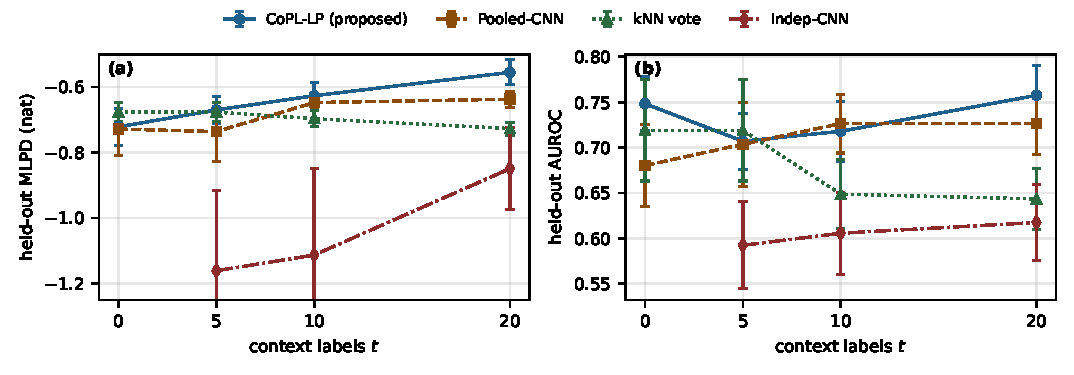
\includegraphics[width=\columnwidth]{figures/fig_curves.pdf}
\caption{Held-out (a) MLPD and (b) AUROC against the context budget $t$ (macro means with occupant-level standard errors; at $t=20$ the five long streams). The proposed rule overtakes the pooled classifier from five labels on and is $0.08$ nat ahead at twenty; the kNN vote, which uses no context, is the best predictor at the cold start.}
\label{fig:curves}
\end{figure}

Table~\ref{tab:main} and Fig.~\ref{fig:curves} report the main comparison.

\emph{Cold start.} With no personal labels the proposed model and the pooled classifier are indistinguishable in MLPD ($-0.722$ against $-0.728$), and the context-free kNN vote is better than both ($-0.677$, paired difference to \method{} $-0.044\pm0.051$). The kNN vote is a conservative predictor: its Laplace-smoothed probabilities are never extreme, which the log score rewards on occupants whose holdout is unpredictable. The reward model with a mean embedding discriminates best (AUROC $0.748$) but is under-confident (ECE $0.29$).

\emph{Personalization.} From five labels on the proposed rule is ahead of the pooled classifier at every budget, and the margin grows with $t$: $+0.066$, $+0.021$, $+0.082$, and $+0.089$ nat at $t=5$, $10$, $20$, and the full context (occupant-level paired differences, Table~\ref{tab:main} footnote). At $t=20$ the difference is two occupant-level standard errors over the five long streams, and the paired change in summed log predictive density is positive for four of them (E2 $+60\pm9$, E3 $+21\pm8$, E4 $+10\pm4$, E5 $+5\pm4$) and negative for E1 at that budget ($-16\pm7$) but positive for E1 at $t=5$ ($+34$) and at the full context ($+32$). The gain appears first in probability quality (Brier $0.186$ against $0.223$, ECE $0.125$ against $0.210$ at $t=20$) and only then in ranking (AUROC $0.758$ against $0.726$): the population already orders the episodes reasonably, and the personal labels mainly tell the model how strongly to commit. Personalization without transfer fails at these budgets; the independent network is worse than the cold start at every $t\le20$. Seed-to-seed variation of the proposed model is $0.011$--$0.025$ nat within a fold, below the occupant-level standard errors.

\begin{table}[t]
\caption{Ablation (Held-Out MLPD, 10 Folds, One Seed)}
\label{tab:ablation}
\centering
\setlength{\tabcolsep}{3.5pt}
\footnotesize
\begin{tabular}{lccccc}
\toprule
Variant & $t=0$ & $t=5$ & $t=10$ & $t=20$ & $n_{\mathrm{ctx}}$ \\
\midrule
\method{} (full model)              & $-0.705$ & $-0.667$ & $-0.629$ & $\mathbf{-0.561}$ & $-0.632$ \\
no adaptation (cold start kept)     & $-0.717$ & $-0.717$ & $-0.684$ & $-0.702$ & $-0.717$ \\
vote, CoPL original \eqref{eq:vote-users} & $-0.711$ & $-0.701$ & $-0.659$ & $-0.644$ & $-0.678$ \\
vote, degree-normalized ($\alpha=1$) & $-0.706$ & $-0.697$ & $-0.662$ & $-0.658$ & $-0.634$ \\
no item--item propagation           & $-0.713$ & $-0.673$ & $-0.633$ & $-0.553$ & $-0.642$ \\
no mixture-consistent training      & $-0.779$ & $-0.735$ & $-0.692$ & $-0.615$ & $-0.680$ \\
no calibration (AUROC selection)    & $-0.709$ & $-0.678$ & $-0.649$ & $-0.570$ & $-0.648$ \\
oracle embedding (upper bound)      & --       & --       & --       & --       & $-0.614$ \\
\bottomrule
\end{tabular}
\\[2pt]
{\footnotesize The full-model row is the first seed of Table~\ref{tab:main}. The vote rows use the temperatures that were tuned for the vote ($\tau=0.5$ and $1$). The oracle conditions the reward model on the held-out occupant's own embedding, obtained by adding her context labels to the population graph.}
\end{table}

\begin{figure}[t]
\centering
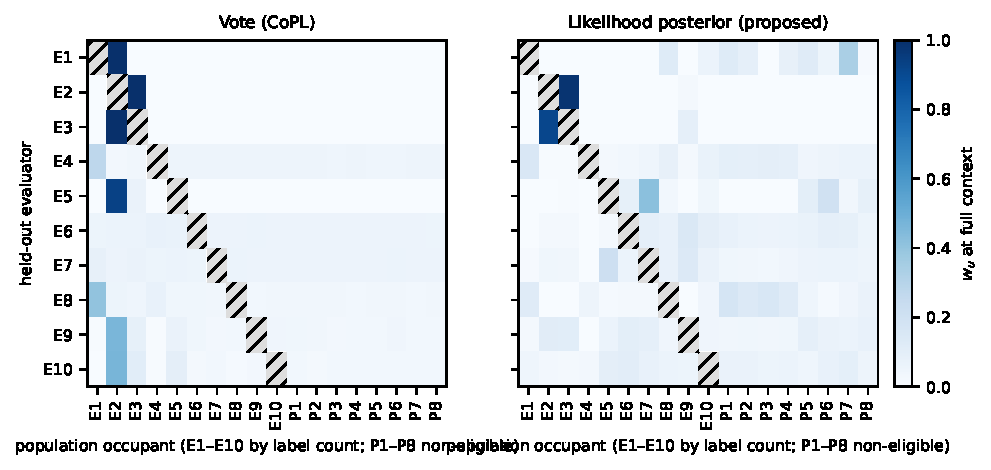
\includegraphics[width=\columnwidth]{figures/fig_wu.pdf}
\caption{Adaptation weights $w_u$ at the full context for each held-out occupant (rows) over the population occupants (columns; E1--E10 ordered by label count, P1--P8 the non-eligible occupants; the hatched cell is the occupant's own, absent from her population). The vote (left) concentrates on the most-labeled population occupant in every row. The likelihood posterior (right) concentrates where the labels agree (E2 and E3, both 76\% good, select each other) and stays spread where no population occupant explains the labels.}
\label{fig:wu}
\end{figure}

\emph{Ablation (Table~\ref{tab:ablation}).} Adaptation is worth $0.14$ nat at $t=20$ over keeping the cold start. The likelihood posterior is ahead of both vote rules by $0.08$--$0.10$ nat at $t=20$; the degree-normalized vote is better than the original at the full context and no better at $t=20$, which is the pattern of Section~\ref{sec:vote}. Removing the item--item term from the graph propagation changes nothing (the embeddings $e_u$ of a star graph are determined by each user's own items either way), and the same holds for the sparsification rule and $k$ of the item graph: in the vote-based run, $24$ combinations of four rules and $k$ from $5$ to $100$ lay within $\pm0.01$ nat of each other at every budget. Mixture-consistent training is necessary at every budget and most at the cold start ($-0.78$ against $-0.71$), where the mean embedding is queried. Calibrated selection matters up to $t=10$; at $t=20$ the evidence is strong enough that the uncalibrated model recovers. The oracle embedding is only $0.02$ nat ahead of the proposed rule at the full context: the adaptation nearly reaches what the reward model can do with the right embedding.

\emph{Adaptation weights (Fig.~\ref{fig:wu}).} The likelihood posterior selects by agreement rather than by size: E2 and E3, who share a base rate of $76\%$ good judgments, select each other with weight above $0.9$; E4 (24\% good) stays spread over several occupants; E1 moves to a non-eligible occupant with weight $0.34$ and reaches $-0.57$ nat, against $-0.62$ for the pooled classifier and $-0.55$ for the oracle. Short streams keep nearly uniform weights, which is the correct behavior when few labels do not single out a population occupant.

\emph{Short streams.} For the five occupants with $10$ to $35$ labels the outcome is mixed at the full context: E9 and E10 gain substantially over the pooled classifier ($-0.87$ against $-1.55$, $-0.57$ against $-0.62$), E6 and E7 lose $0.03$ nat, and E8 loses $0.17$ nat. The inner search sees mostly long streams and selected $\tau=1$; in a grid over $\tau$ evaluated after the fact, $\tau=10$ limits the worst short-stream loss to $0.05$ nat at the price of $0.05$ nat at $t=20$ on the long streams. A context-length-dependent temperature is the obvious refinement and is left for future work.

\section{Discussion and Limitations}
\label{sec:discussion}

\textbf{Adaptation is a selection problem.} Three observations recur across the experiment. The upper bound of conditioning the reward model on a population embedding is high (the oracle beats the pooled classifier by $0.10$ nat at the full context), the best adaptation setting chosen per fold would exceed even that bound, and the single rule that fails is the one that measures agreement indirectly. Few-label personalization in this pipeline is therefore less about the representation than about how the few labels select among population users, and a rule that scores users on the same labels with the same probabilistic model is the natural choice. The scale of the evidence matters: the log-likelihood is in nats, which is why calibration enters the ablation and why $\tau$ has a Bayesian reading.

\textbf{What the graph is for.} On star-structured data the item graph does two things: it defines the kNN vote baseline, and it is an input to the graph propagation that produces $e_u$. Neither its sparsification nor the item--item term in the propagation affects the outcome. The encoder matters for the first role, where a fixed scattering representation beats learned autoencoders by a wide margin; for the second, the user embeddings are essentially per-user summaries of each user's own labeled items.

\textbf{Limitations.} The population has $18$ occupants and the $t=20$ results rest on five long streams; occupant-level intervals are wide by construction, and we have drawn conclusions only where the paired occupant-level differences and the episode-level differences agree. Occupants with around thirty labels are the ones personalization is meant for, and for them the results are mixed; a temperature that depends on the context length, or an inner search that weights short streams, is the next step. The cold start is no better than a pooled classifier and worse than a context-free kNN vote; the proposed rule pays off from five labels on. Adaptation assumes that the new occupant is approximately a mixture of population occupants; an occupant unlike anyone in the population has a low oracle bound to begin with (E8, $-0.86$). The label is a single good/bad judgment, the context of the feedback is not modeled, and the loop from the personalized predictor to a controller is outside this paper.

\section{Conclusion}
\label{sec:conclusion}

We transferred collaborative preference learning to in-vehicle ride feedback and found its test-time adaptation to be the weak link: on data where every item belongs to one user, the graph vote has a degree bias that no normalization repairs. Scoring population users by the reward model's likelihood of the new occupant's labels and tempering the resulting posterior removes the bias without a graph, improves the held-out log predictive density after twenty labels by $0.08$ nat over a fine-tuned pooled classifier and by $0.09$ nat over the vote, and comes within $0.02$ nat of the oracle embedding. The pipeline needs mixture-consistent training and calibration of the reward model, but not item--item propagation, graph sparsification, or a learned encoder. The adaptation step costs one forward pass per population user and label and can run in the vehicle.

\section*{Acknowledgment}
\draftnote{Funding, data-collection acknowledgments, conflicts of interest.}

\bibliographystyle{IEEEtran}
\bibliography{refs}

\end{document}
